\chapter{Resultados} \label{cap:resultados}

Nessa sessão, os resultados serão dados em termos da área medida entre a diferença da \ac{PDF} real e a estimada, como previamente mencionado. Nas figuras que seguem , os valores serão mostrados no eixo vertical, nomeado de \textit{Erro}. O eixo horizontal mostra quatro perspectivas diferentes: Probabilidade, Eixo $ x $ (que seria os valores aleatórios da variável), Primeira derivada, e segunda derivada. Essas perspectivas diferentes irão permitir um melhor entendimento das características de cada método. Cada gráfico será completado com 100 pontos de dados, cada um representando o erro medido encontrado em cada \ac{RoI} (Contudo, nessa sessão, serão considerados 100 \ac{RoI} ao invés de 20 como mostrado na Figura~\ref{fig:error}). Essa sessão será será dividida em três análises diferentes. Sessão~\ref{cap:interp_neares} analisa a estimação de erro quando a interpolação pelo vizinho mais próximo é usada; Sessão~\ref{cap:interp_lin} avalia para a interpolação linear; e a Sessão~\ref{cap:interp_neares} insere problemas de \textit{outliers}. Quando \textit{outliers} são gerados, o desempenho de alguns métodos de discretização podem ser altamente degradados em comparação com outros, sendo uma questão importante a ser analisada.

\section{Estimação de erro pela interpolação do vizinho mais próximo} \label{cap:interp_neares}
A interpolação pelo vizinho mais próximo basicamente atribui o valor vizinho mais próximo ao valor da probabilidade da variável aleatória que será estimada. Portanto, o erro de estimação será proporcional à sua distância da amostra mais próxima. Tal método de interpolação produz um erro diretamente proporcional à primeira derivada \cite{gurevich1966integral}. Analisando as Figura~\ref{fig:12a} e \ref{fig:12b} pode-se inferir que: 

\begin{figure}[H]
	\centering
	\begin{subfigure}[b]{0.45\textwidth}
		\centering 
		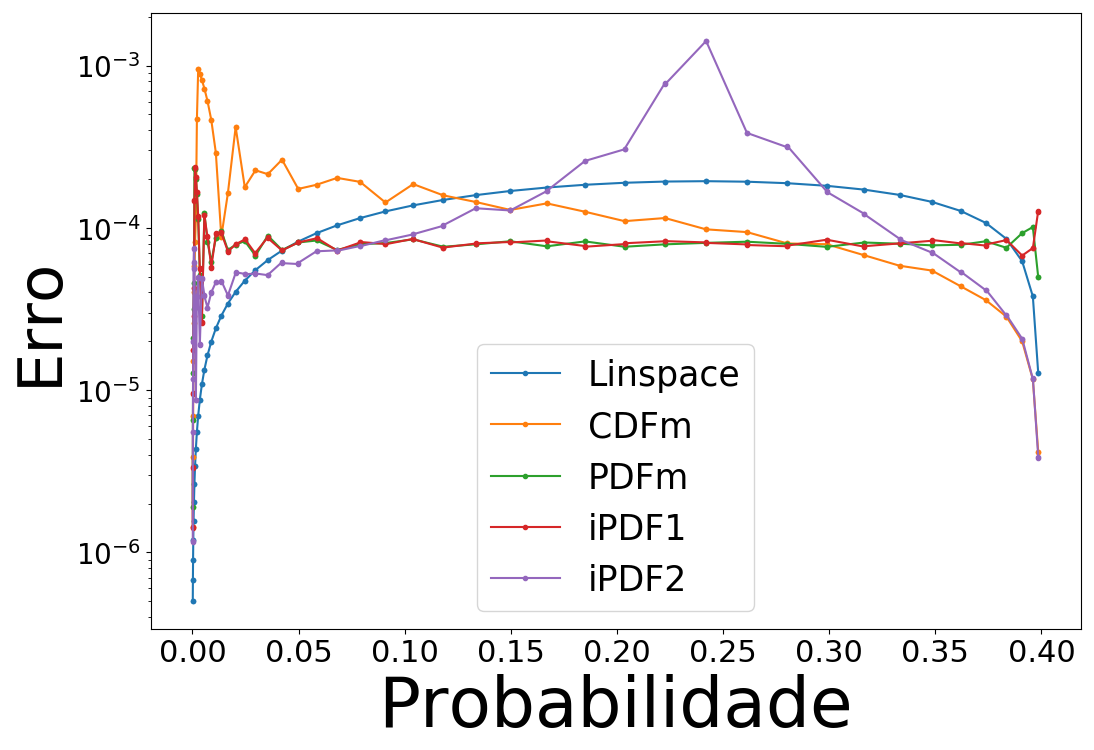
\includegraphics[width=\textwidth]{./figuras/error_normal_nearest_Probabilidade}
		\caption{}
		\label{fig:12a}
	\end{subfigure}
	\hfill
	~ %add desired spacing between images, e. g. ~, \quad, \qquad, \hfill etc. 
	%(or a blank line to force the subfigure onto a new line)
	\begin{subfigure}[b]{0.45\textwidth}
		\centering 
		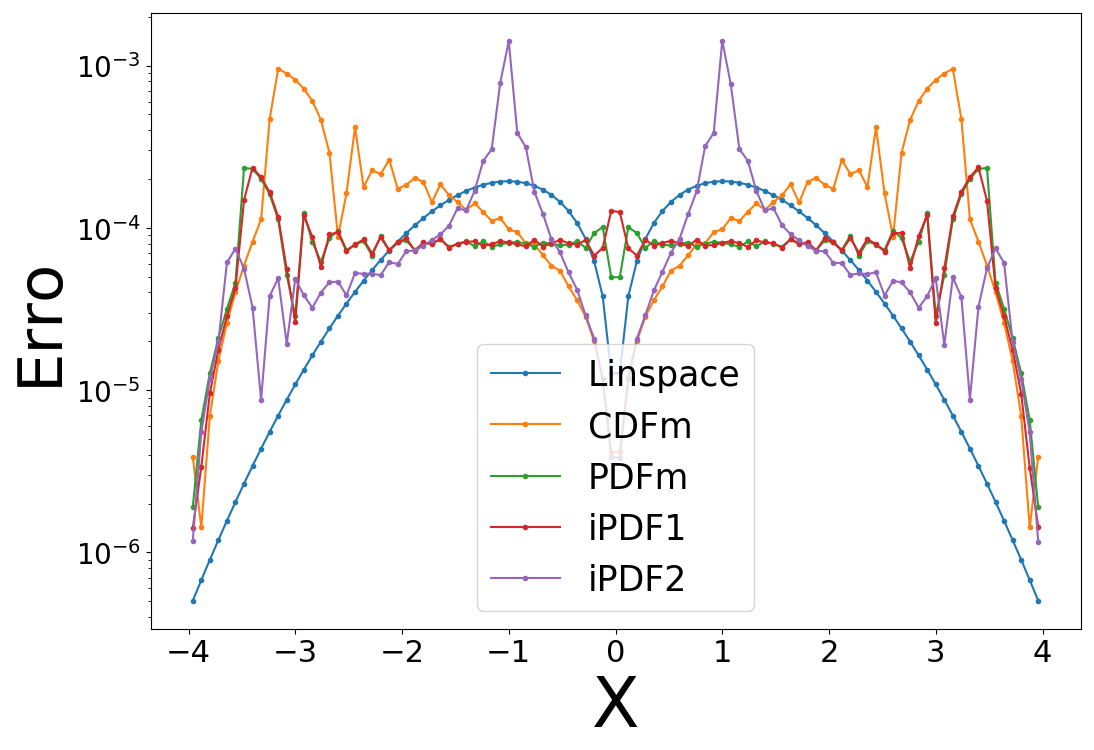
\includegraphics[width=\textwidth]{./figuras/error_normal_nearest_X}
		\caption{}
		\label{fig:12b}
	\end{subfigure}
	%\vskip\baselineskip
	~ %add desired spacing between images, e. g. ~, \quad, \qquad, \hfill etc. 
	%(or a blank line to force the subfigure onto a new line)
	\begin{subfigure}[b]{0.45\textwidth}
		\centering 
		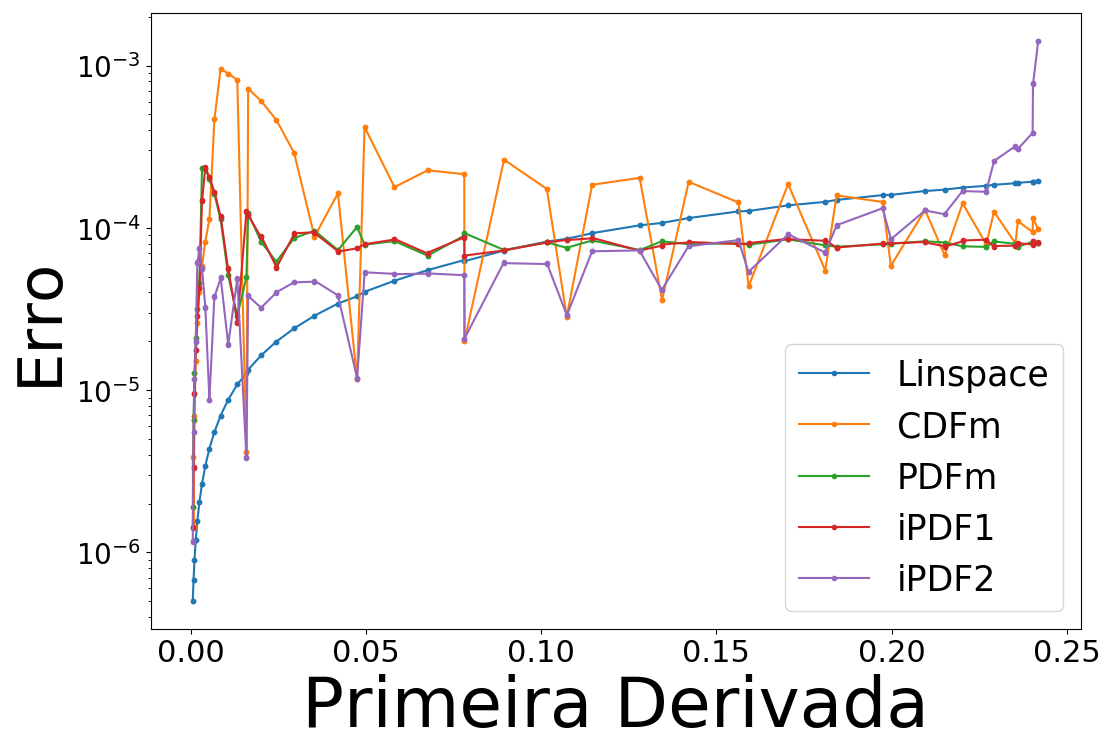
\includegraphics[width=\textwidth]{./figuras/error_normal_nearest_Primeira Derivada.png}
		\caption{}
		\label{fig:12c}
	\end{subfigure}
	\hfill
	\begin{subfigure}[b]{0.45\textwidth}
		\centering 
		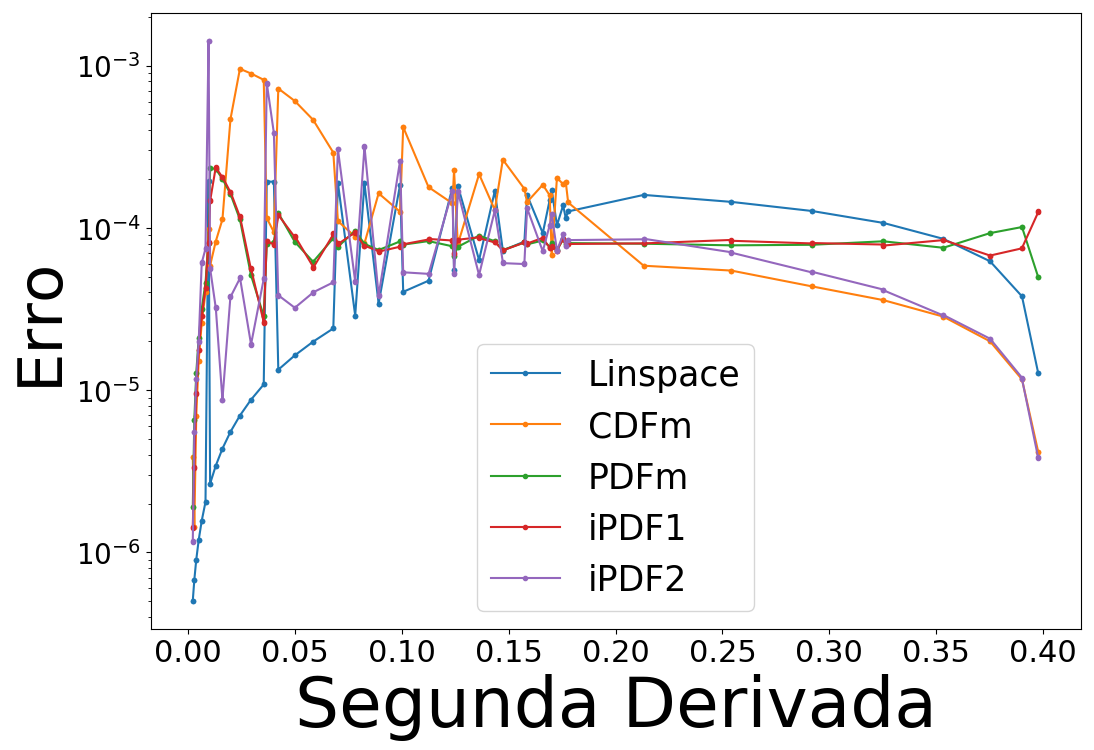
\includegraphics[width=\textwidth]{./figuras/error_normal_nearest_Segunda Derivada.png}
		\caption{}
		\label{fig:12d}
	\end{subfigure}
	\caption{Caso representativo com 200 pontos, 100 \ac{RoI} e usando a interpolação pelo vizinho mais próximo.}
	\label{fig:12}
\end{figure}

\section{Estimação de erro pela interpolação linear} \label{cap:interp_lin}

\begin{figure}[H]
	\centering
	\begin{subfigure}[b]{0.45\textwidth}
		\centering 
		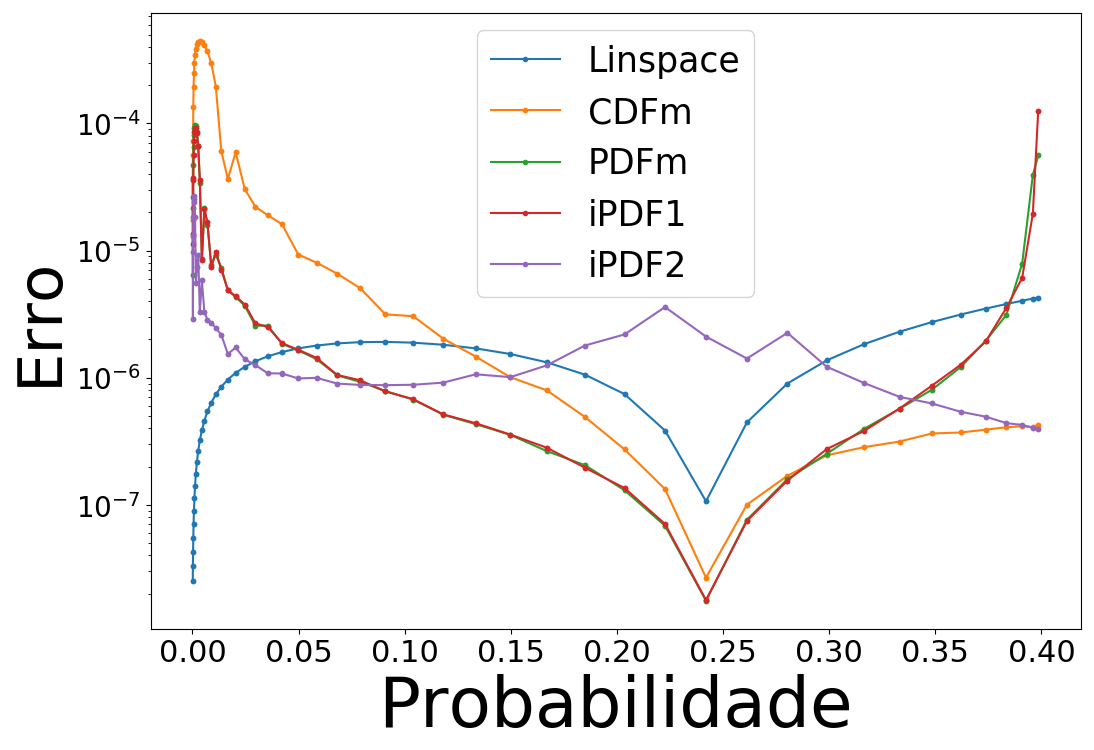
\includegraphics[width=\textwidth]{./figuras/error_normal_linear_Probabilidade}
		\caption{}
		\label{fig:11a}
	\end{subfigure}
	\hfill
	~ %add desired spacing between images, e. g. ~, \quad, \qquad, \hfill etc. 
	%(or a blank line to force the subfigure onto a new line)
	\begin{subfigure}[b]{0.45\textwidth}
		\centering 
		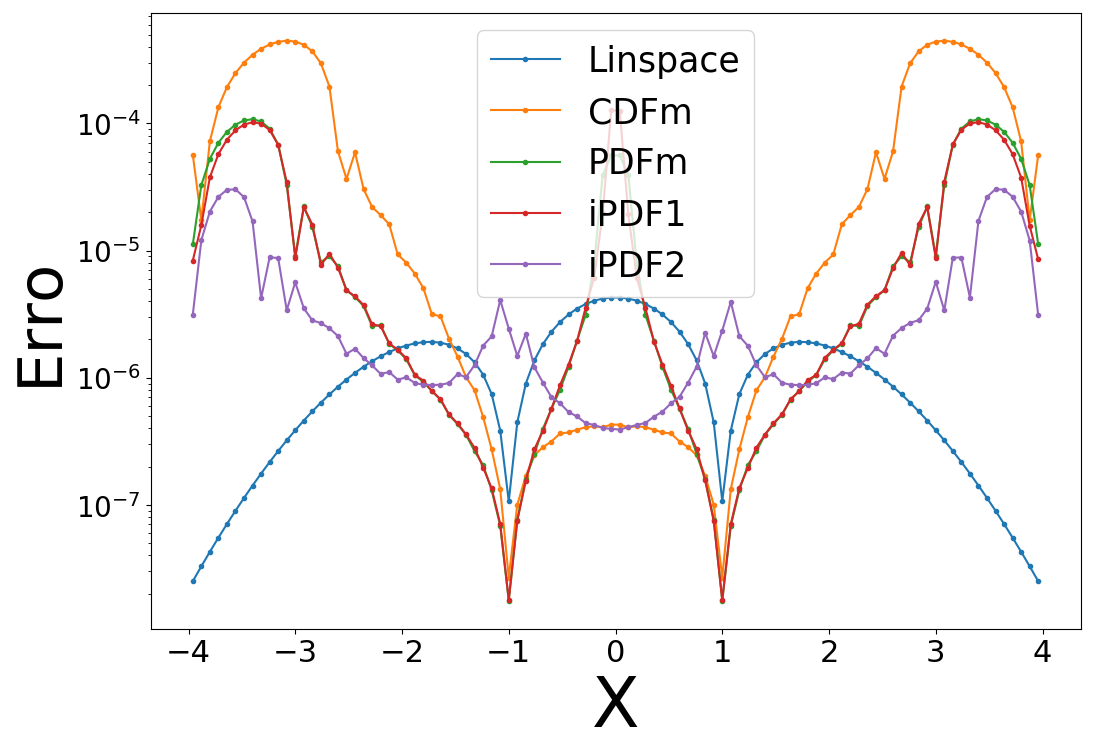
\includegraphics[width=\textwidth]{./figuras/error_normal_linear_X}
		\caption{}
		\label{fig:11b}
	\end{subfigure}
	%\vskip\baselineskip
	~ %add desired spacing between images, e. g. ~, \quad, \qquad, \hfill etc. 
	%(or a blank line to force the subfigure onto a new line)
	\begin{subfigure}[b]{0.45\textwidth}
		\centering 
		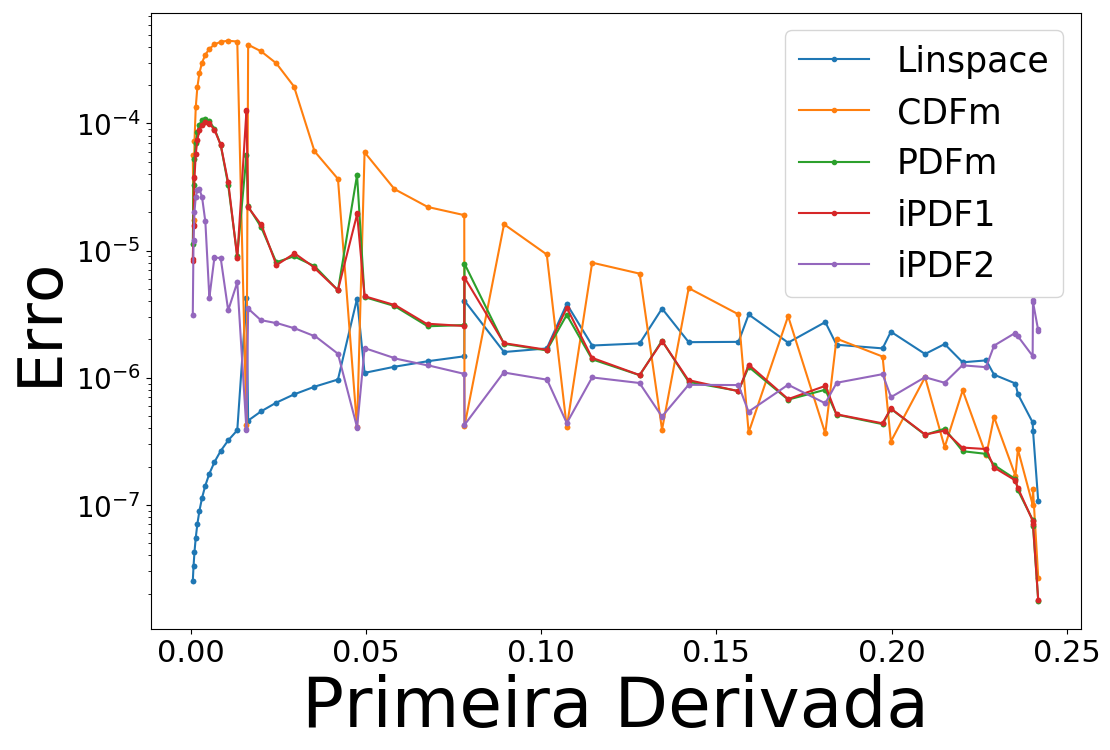
\includegraphics[width=\textwidth]{./figuras/error_normal_linear_Primeira Derivada.png}
		\caption{}
		\label{fig:11c}
	\end{subfigure}
	\hfill
	\begin{subfigure}[b]{0.45\textwidth}
		\centering 
		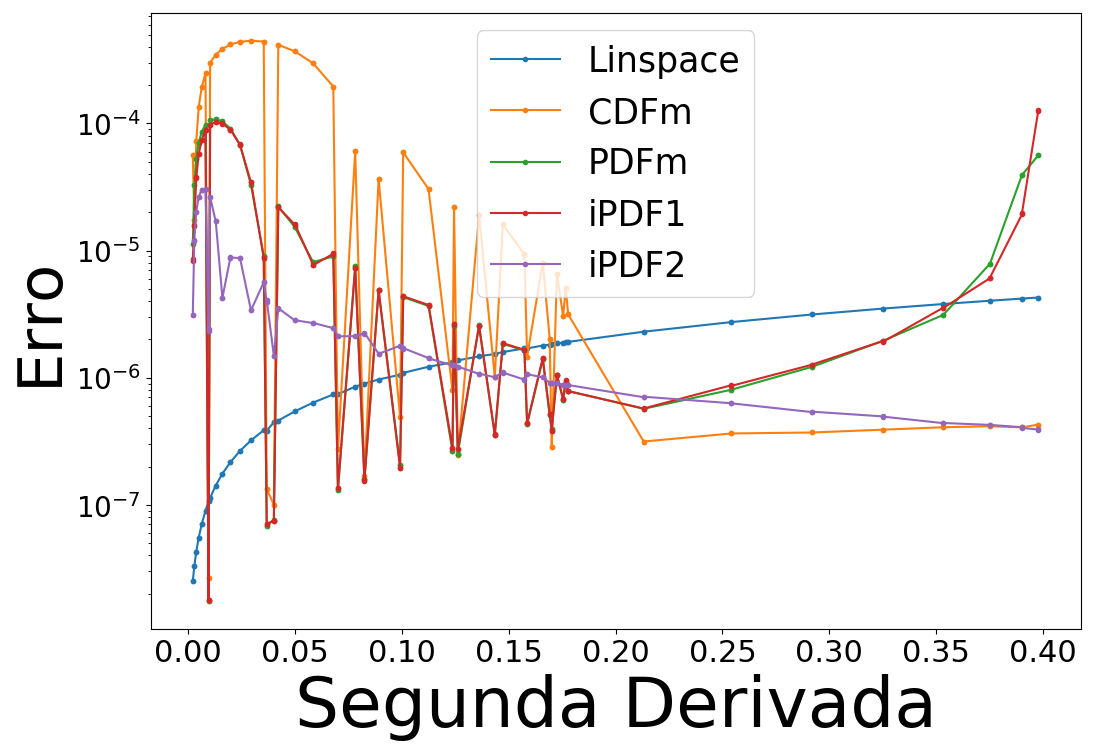
\includegraphics[width=\textwidth]{./figuras/error_normal_linear_Segunda Derivada.png}
		\caption{}
		\label{fig:11d}
	\end{subfigure}
	
	\caption{Caso representativo com 200 pontos, 100 \ac{RoI} e usando a interpolação linear.}\label{fig:11}
\end{figure}

\section{Estimação de erro considerando \textit{outliers}} \label{cap:erro_out}